\documentclass[11pt]{article}
\usepackage[margin=1in]{geometry}
\usepackage{graphicx}
\usepackage{amsmath}
\usepackage{hyperref}
\usepackage{enumitem}
\usepackage{caption}
\usepackage{placeins}
\usepackage[most]{tcolorbox}

\title{CMPT 742 Assignment 3 Report}
\author{Yueyang Li\\yla919@sfu.ca\\Student ID: 301657120}
\date{\today}

\begin{document}

\maketitle

\section{Introduction}
A object detection model trained on a limited sized dataset based on SSD architecture

\section{Demo Test}
This section presents qualitative outputs on ten external images. Each row shows two resized outputs placed side-by-side for easy comparison.

\begin{figure}[h]
    \centering
    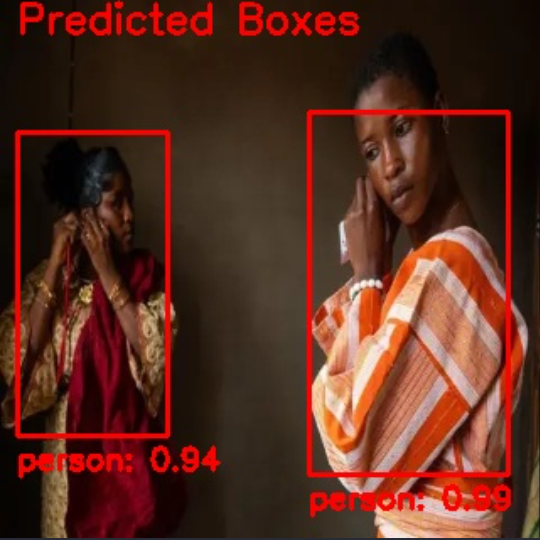
\includegraphics[width=0.4\textwidth]{images/00.png}
    \hspace{0.5cm}
    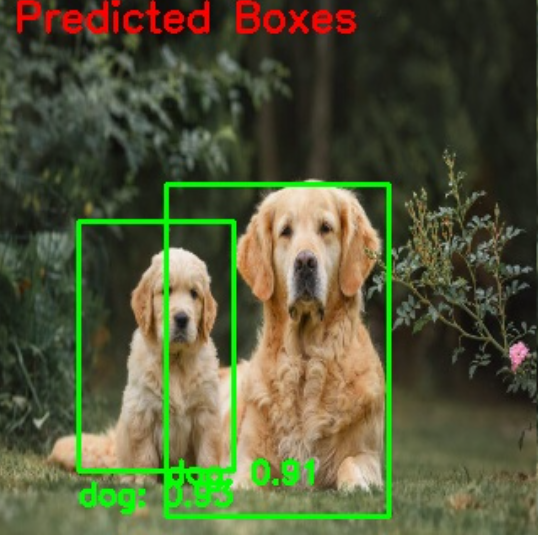
\includegraphics[width=0.4\textwidth]{images/01.png}
    \caption{Demo Test samples 1--2.}
    \label{fig:demo_pair_1}
\end{figure}

\begin{figure}[h]
    \centering
    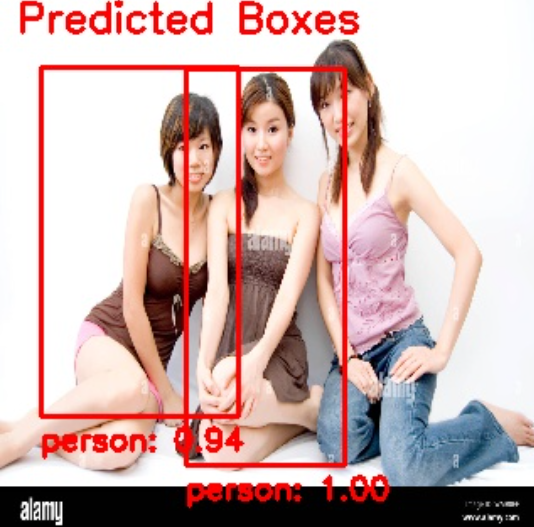
\includegraphics[width=0.4\textwidth]{images/02.png}
    \hspace{0.5cm}
    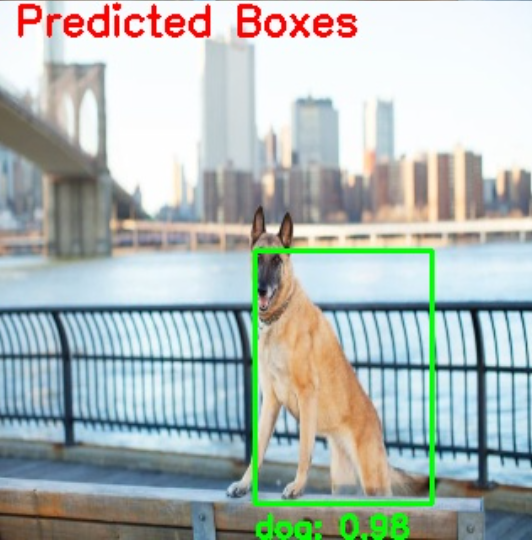
\includegraphics[width=0.4\textwidth]{images/03.png}
    \caption{Demo Test samples 3--4.}
    \label{fig:demo_pair_2}
\end{figure}

\begin{figure}[h]
    \centering
    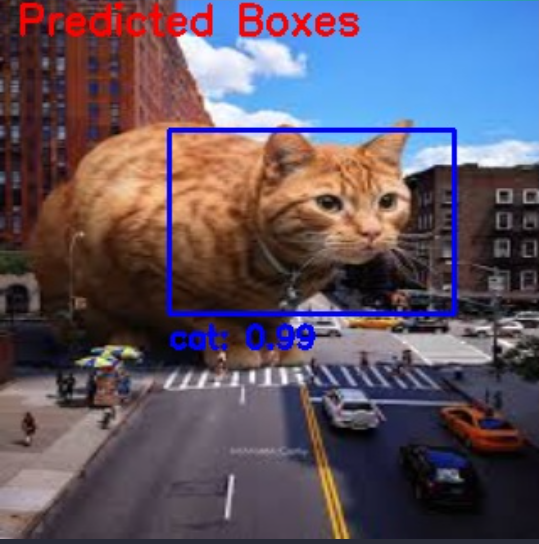
\includegraphics[width=0.4\textwidth]{images/04.png}
    \hspace{0.5cm}
    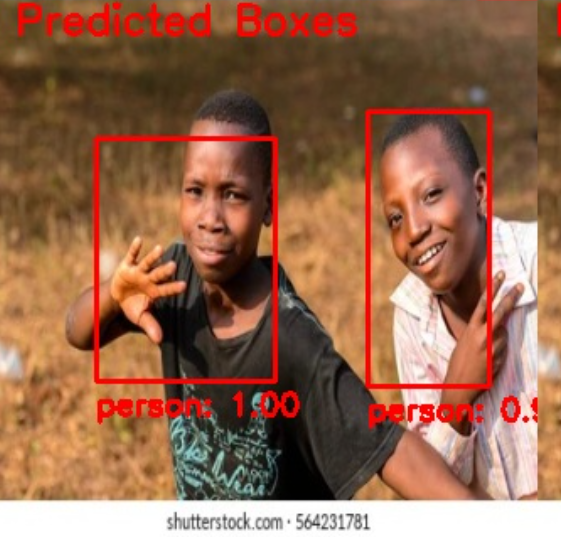
\includegraphics[width=0.4\textwidth]{images/05.png}
    \caption{Demo Test samples 5--6.}
    \label{fig:demo_pair_3}
\end{figure}

\begin{figure}[h]
    \centering
    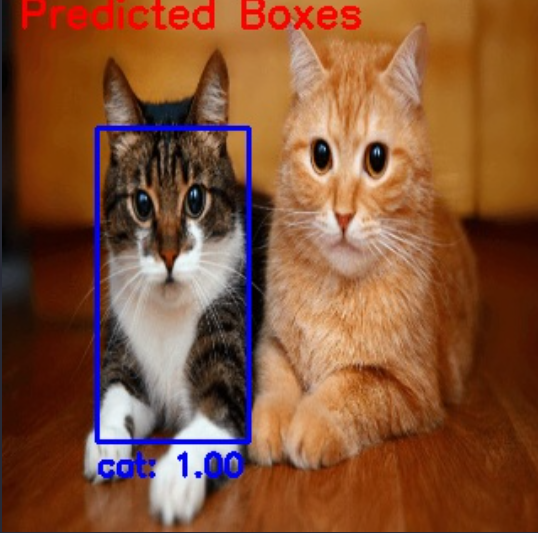
\includegraphics[width=0.4\textwidth]{images/06.png}
    \hspace{0.5cm}
    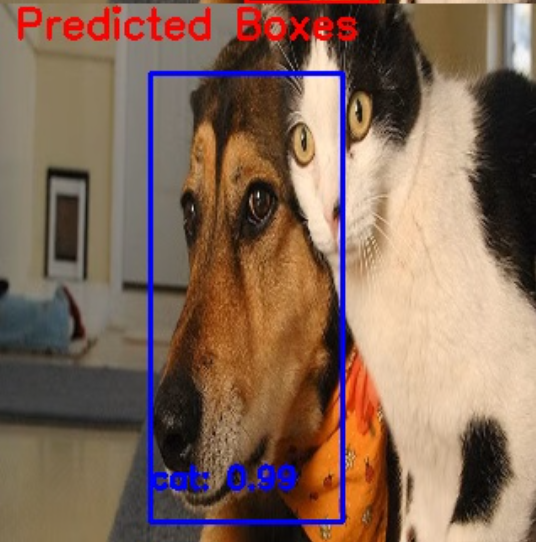
\includegraphics[width=0.4\textwidth]{images/07.png}
    \caption{Demo Test samples 7--8.}
    \label{fig:demo_pair_4}
\end{figure}

\begin{figure}[h]
    \centering
    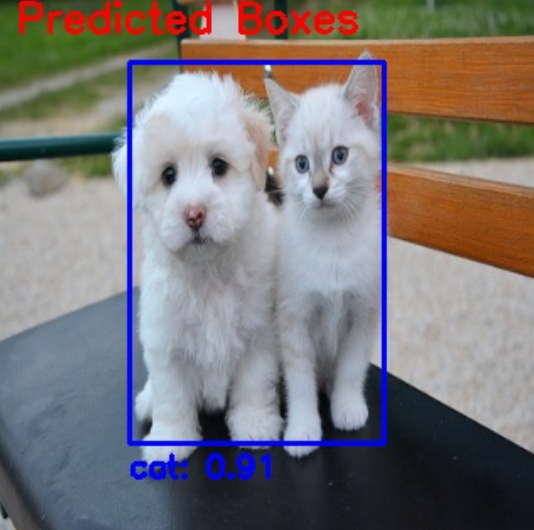
\includegraphics[width=0.4\textwidth]{images/08.png}
    \hspace{0.5cm}
    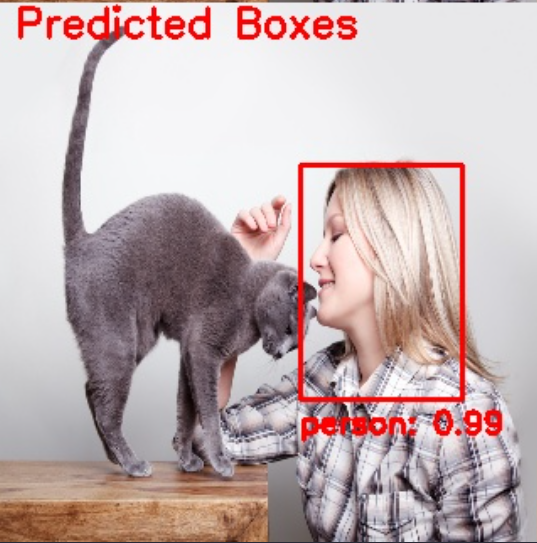
\includegraphics[width=0.4\textwidth]{images/09.png}
    \caption{Demo Test samples 9--10.}
    \label{fig:demo_pair_5}
\end{figure}

\FloatBarrier

\section{Review}
\begin{tcolorbox}[colback=white,colframe=black,title=Performance Reflection]
Where and why does your model work and not work on the images you chose?
\end{tcolorbox}

\begin{itemize}
    \item My model performs fairly well for the single person, multiple person, single dog, multiple dogs and single cat scenes. However, it performs poorly for mixing cats, dogs, and human scenes.
    \item There are two major reasons that I believe might be the major issues that are causing the model to perform badly in these scenes:
    \begin{itemize}
        \item The dataset is heavily person-class-skewed. Among the 6{,}392 training annotations stored in \texttt{data/train/annotations}, 5{,}102 are labeled as ``person'' while only 992 and 886 correspond to ``cat'' and ``dog'' respectively. With more than 80\% of anchors supervised by a single class, the classifier learns to over-trust the person prior, so mixed scenes trigger person boxes everywhere and suppress minority classes even when their local visual cues are strong.
        \item The SSD head defined in \texttt{model.py} is also simplistic: it only exposes four prediction scales (10$\times$10, 5$\times$5, 3$\times$3, 1$\times$1) and each cell emits four nearly square default boxes. This limited anchor bank struggles when images contain multiple elongated objects (standing people plus crouching pets) because no aspect-ratio-specific anchors remain after the feature pyramid is repeatedly downsampled. Once the matching step fails to find high-IoU anchors for cats or dogs, the loss provides almost no localization signal for those classes in the same frame.
    \end{itemize}
\end{itemize}

\section{Improvement}
\begin{tcolorbox}[colback=white,colframe=black,title=Improvement]
What can be done to improve the result 
\end{tcolorbox}

\begin{itemize}
    \item Train the model on a larger, more balanced dataset
    \item train the model with better hyper-parameters
    \item Better data augmentation techniques can be applied to improve the training result beyond the current one based on albumentation library

\end{itemize}

\section{Confidence Threshold}

\section{Confidence Threshold}
\begin{tcolorbox}[colback=white,colframe=black,title=Improvement]
What is the best confidence threshold for your your model for the 10 images you chose. You can get this value by running the model at different thresholds and judging the predictions visually. 
\end{tcolorbox}

The best \textbf{confidence level} for my model for the 10 images is:\\
\begin{center}
    \textbf{0.9}
\end{center}
\begin{figure}[h]
    \centering
    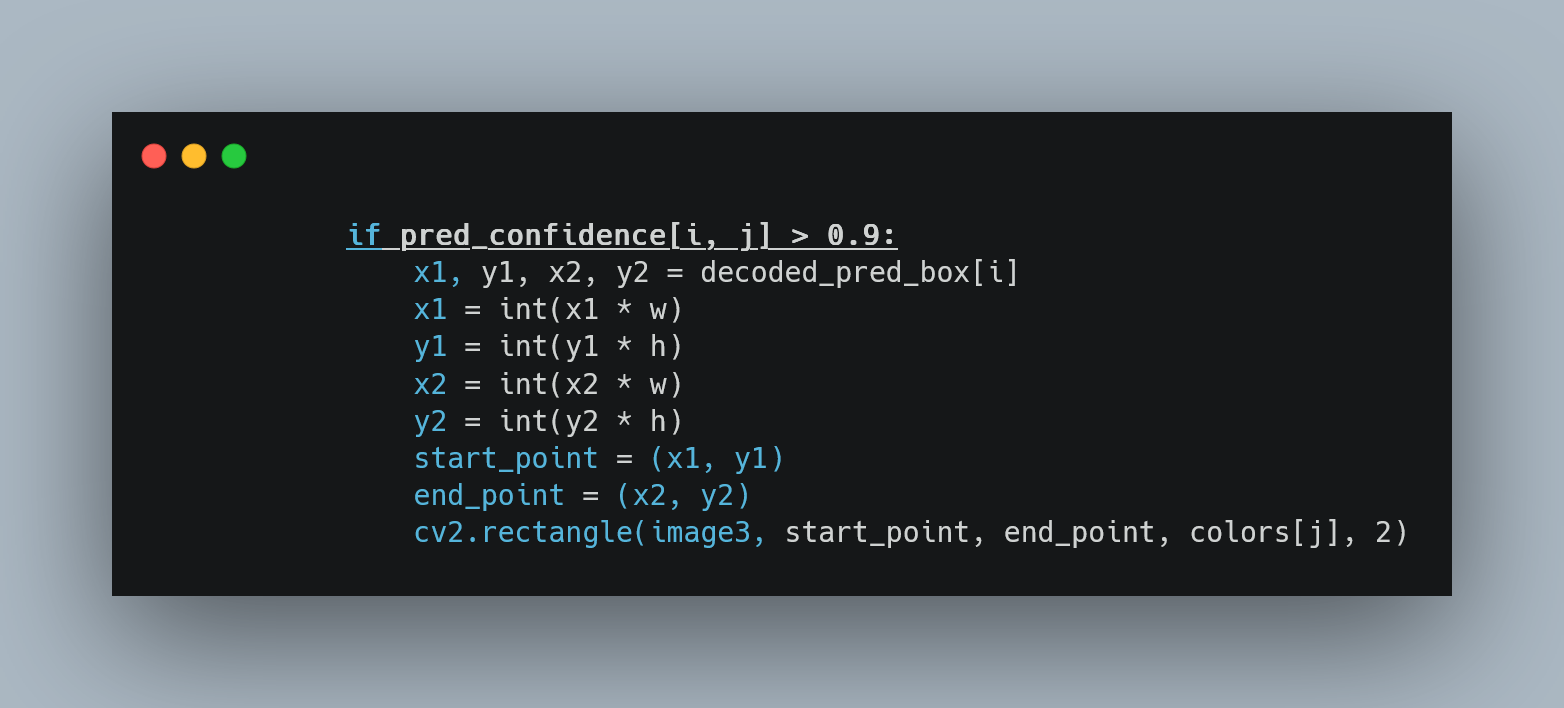
\includegraphics[width=0.8\textwidth]{images/confidence.png}
    \label{fig:demo_pair_5}
\end{figure}


\section{Instructions while completing the project}

\begin{tcolorbox}[colback=white, colframe=black,title=Instruction 1]

\begin{verbatim}
# TODO: save predicted bounding boxes and classes to a txt
\end{verbatim}

\end{tcolorbox}

By running \verb|run.ps1| with \verb|-Mode test|, in the \verb|output/predict| folder, you can get the of the predictions in names of \verb*|predictions_xxx.txt| file. All predicted bounding boxes laying over the original image can be found in \verb*|output/images|folder. \\
Here are some of the examples output that you can find in the folder

\begin{figure}[h]
    \centering
    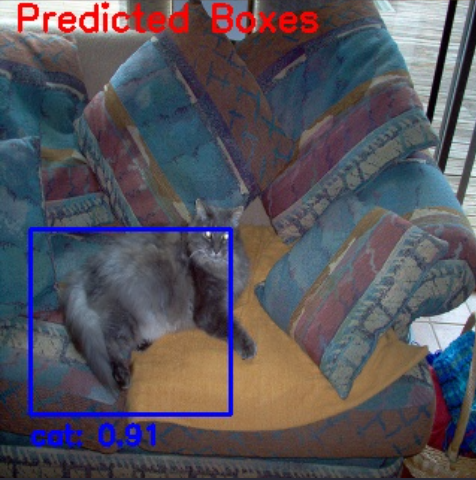
\includegraphics[width=0.4\textwidth]{images/test_exp_01.png}
    \hspace{0.5cm}
    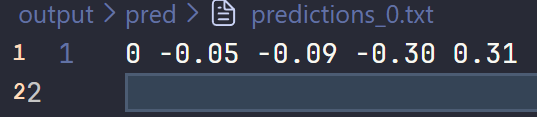
\includegraphics[width=0.4\textwidth]{images/test_exp_01_txt.png}
    \caption{demo test output 1}
    \label{fig:demo test output 1}
\end{figure}

\begin{figure}[h]
    \centering
    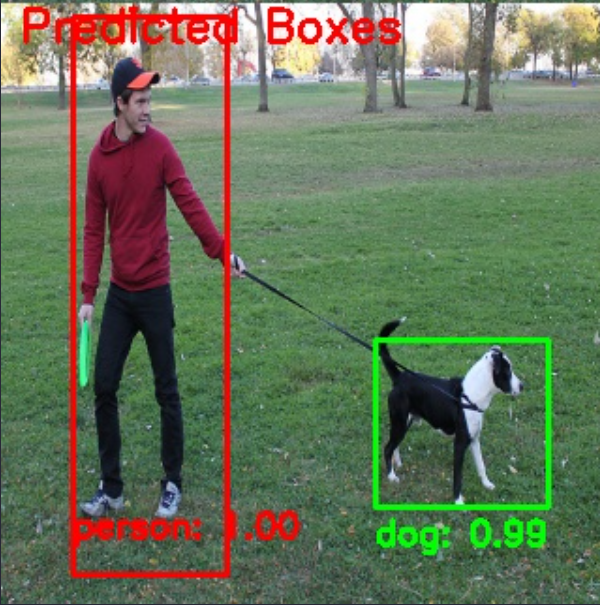
\includegraphics[width=0.4\textwidth]{images/test_exp_02.png}
    \hspace{0.5cm}
    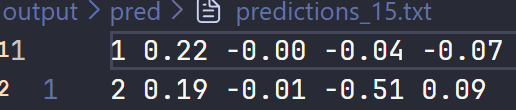
\includegraphics[width=0.4\textwidth]{images/test_exp_02_txt.png}
    \caption{demo test output 2}
    \label{fig:demo test output 2}
\end{figure}


\begin{tcolorbox}[colback=white, colframe=black,title=Instruction 2]
mAP 
\end{tcolorbox}

By running run.ps1 -Mode map, a map plot will be generated. This is the Precision-Recall-Curve for all classes.
 \begin{figure}[h]
    \centering
    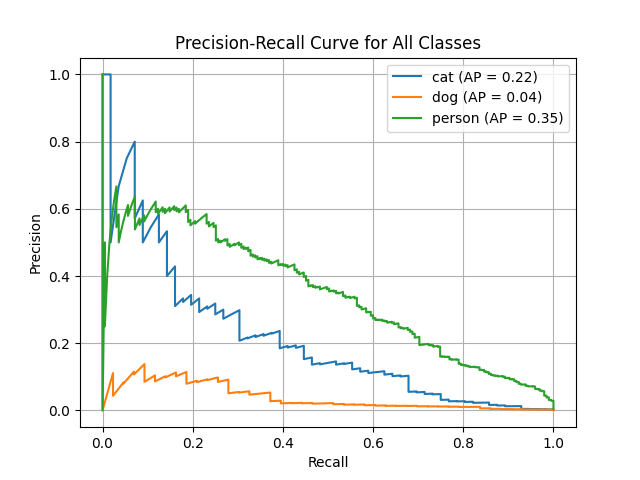
\includegraphics[width=0.6\textwidth]{images/mAP-precision-recall-curve.png}
    \caption{Precision Recall Curve}
    \label{fig:demo test output 2}
\end{figure}

\end{document}
